	\section{Εισαγωγή}

\section{Τι είναι ο κατακερματισμός;}
Ο κατακερματισμός (hashing) είναι μια μέθοδος που επιτυγχάνει ταχύτατη αποθήκευση και αναζήτηση δεδομένων. Σε ένα σύστημα κατακερματισμού τα δεδομένα αποθηκεύονται σε έναν πίνακα που ονομάζεται πίνακας κατακερματισμού (hash table). Εφαρμόζοντας στο κλειδί κάθε εγγραφής που πρόκειται να αποθηκευτεί ή να αναζητηθεί τη συνάρτηση κατακερματισμού (hash function) προσδιορίζεται μονοσήμαντα η θέση του πίνακα στην οποία τοποθετούνται τα δεδομένα της εγγραφής.
Μια καλή συνάρτηση κατακερματισμού θα πρέπει να κατανέμει τα κλειδιά στα κελιά του πίνακα κατακερματισμού όσο πιο ομοιόμορφα γίνεται και να είναι εύκολο να υπολογιστεί.

\begin{figure}[h]
\centering
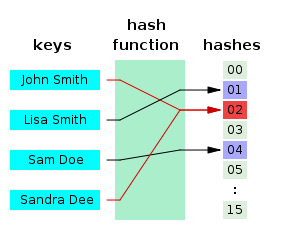
\includegraphics{HashTable.png}
\caption{}
\label{fig:hashtable1}
\end{figure}

Είναι επιθυμητό το παραγόμενο αποτέλεσμα από τη συνάρτηση κατακερματισμού να εξαρτάται από το κλειδί στο σύνολό του.

Οι πίνακες κατακερματισμού είναι ιδιαίτερα κατάλληλοι για εφαρμογές στις οποίες πραγματοποιούνται συχνές αναζητήσεις εγγραφών με δεδομένες τιμές κλειδιών. Ωστόσο, οι πίνακες κατακερματισμού έχουν και μειονεκτήματα καθώς είναι δύσκολο να επεκταθούν από τη στιγμή που έχουν δημιουργηθεί και μετά. Επίσης, η απόδοσή των πινάκων κατακερματισμού υποβαθμίζεται καθώς οι θέσεις τους γεμίζουν με στοιχεία. Συνεπώς, εφόσον ο προγραμματιστής προχωρήσει στη δική του υλοποίηση ενός πίνακα κατακερματισμού είτε θα πρέπει να γνωρίζει εκ των προτέρων το πλήθος των στοιχείων που πρόκειται να αποθηκευτούν είτε όταν αυτό απαιτηθεί να υπάρχει πρόβλεψη έτσι ώστε τα δεδομένα να μεταφέρονται σε μεγαλύτερο πίνακα κατακερματισμού.

Στις περισσότερες εφαρμογές υπάρχουν πολύ περισσότερα πιθανά κλειδιά εγγραφών από ότι θέσεις στο πίνακα κατακερματισμού. Αν για δύο ή περισσότερα κλειδιά η εφαρμογή της συνάρτησης κατακερματισμού δίνει το ίδιο αποτέλεσμα τότε λέμε ότι συμβαίνει σύγκρουση (collision) η οποία θα πρέπει να διευθετηθεί με κάποιο τρόπο. Ειδικότερα, η εύρεση μιας εγγραφής με κλειδί k είναι μια διαδικασία δύο βημάτων:
\begin{itemize}[noitemsep]
\item Εφαρμογή της συνάρτησης κατακερματισμού στο κλειδί της εγγραφής.
\item Ξεκινώντας από την θέση που υποδεικνύει η συνάρτηση κατακερματισμού στον πίνακα κατακερματισμού, εντοπισμός της εγγραφής που περιέχει το ζητούμενο κλειδί (ενδεχόμενα θα χρειαστεί να εφαρμοστεί κάποιος μηχανισμός διευθέτησης συγκρούσεων). 
\end{itemize}

\subsection{Ανοικτή διευθυνσιοδότηση}

\subsection{Κατακερματισμός με αλυσίδες}

\section{Κατακερματισμός με την STL}
Η STL διαθέτει την κλάση std::hash που μπορεί να χρησιμοποιηθεί για την επιστροφή hash τιμών για διάφορους τύπους δεδομένων. Στον ακόλουθο κώδικα παρουσιάζεται η χρήση της 
std::hash.

\lstinputlisting[caption = Παράδειγμα χρήσης της std::hash (stl\_hash.cpp)]{lab07/stl_hash.cpp}

\lstinputlisting[style=DOS]{lab07/stl_hash.out}
 

Επιπλεον, η STL υποστηρίζει δύο βασικές δομές κατακερματισμού το std::unordered\_set και το std::unordered\_map. Το std::unordered\_set υλοποιείται ως ένας πίνακας κατακερματισμού και μπορεί να περιέχει τιμές (κλειδιά) οποιουδήποτε τύπου οι οποίες γίνονται hash σε διάφορες θέσεις του πίνακα κατακερματισμού. Κατά μέσο όρο, οι λειτουργίες σε ένα std::unordered\_set (εύρεση, εισαγωγή και διαγραφή κλειδιού) πραγματοποιούνται σε σταθερό χρόνο O(1). Ένα std::unordered\_set δεν περιέχει διπλότυπα, ενώ αν υπάρχει αυτή η ανάγκη τότε μπορεί να χρησιμοποιηθεί το std::unordered\_multiset. 

Στον κώδικα που ακολουθεί οι χαρακτήρες ενός λεκτικού εισάγονται ένας προς ένας σε ένα std::unordered\_set έτσι ώστε να υπολογιστεί το πλήθος των διακριτών χαρακτήρων του λεκτικού.

\lstinputlisting[caption = Παράδειγμα χρήσης του std::unordered\_set (stl\_unordered\_set.cpp)]{lab07/stl_unordered_set.cpp}

\lstinputlisting[style=DOS]{lab07/stl_unordered_set.out}

To std::unordered\_map αποθηκεύει ζεύγη (κλειδί-τιμή). Το κλειδί αναγνωριζει με μοναδικό τρόπο το κάθε ζεύγος και γίνεται hash σε συγκεκριμένη θέση του πίνακα κατακερματισμού. Όπως και στο std::unordered\_set. κατά μέσο όρο, οι λειτουργίες σε ένα std::unordered\_map πραγματοποιούνται σε σταθερό χρόνο O(1). Η ανάθεση τιμής σε κλειδί μπορεί να γίνει με τους τελεστές = και [] ενώ το πέρασμα από τις τιμές ενός std::unordered\_map μπορεί να γίνει με  iterator ή με range for.
 
\lstinputlisting[caption = Παράδειγμα χρήσης του std::unordered\_map (stl\_unordered\_map.cpp)]{lab07/stl_unordered_map.cpp}

\lstinputlisting[style=DOS]{lab07/stl_unordered_map.out}

\section{Κατακερματισμός και κρυπτογράφηση}

\section{Bloom filters}
A Bloom filter is a space-efficient probabilistic data structure, conceived by Burton Howard Bloom in 1970, that is used to test whether an element is a member of a set. False positive matches are possible, but false negatives are not – in other words, a query returns either "possibly in set" or "definitely not in set". Elements can be added to the set, but not removed (though this can be addressed with a "counting" filter); the more elements that are added to the set, the larger the probability of false positives.

\section{Παραδείγματα}

\subsection{Παράδειγμα 1}
Έστω μια επιχείρηση η οποία επιθυμεί να αποθηκεύσει τα στοιχεία των υπαλλήλων της (όνομα, διεύθυνση) σε μια δομή έτσι ώστε με βάση το όνομα του υπαλλήλου να επιτυγχάνει τη γρήγορη ανάκληση των υπόλοιπων στοιχείων των υπαλλήλων. Στη συνέχεια παρουσιάζεται η υλοποίηση ενός πίνακα κατακερματισμού στον οποίο κλειδί θεωρείται το όνομα του υπαλλήλου και η επίλυση των συγκρούσεων πραγματοποιείται με ανοικτή διευθυνσιοδότηση (open addressing) και γραμμική αναζήτηση (linear probing). Ο πίνακας κατακερματισμού μπορεί να δεχθεί το πολύ 10.000 εγγραφές υπαλλήλων. Στο παράδειγμα χρονομετρείται η εκτέλεση για 2.000, 3.000 και 8.000 υπαλλήλους. Παρατηρείται ότι λόγω των συγκρούσεων καθώς ο συντελεστής φόρτωσης του πίνακα κατακερματισμού αυξάνεται η απόδοση της δομής υποβαθμίζεται.

\lstinputlisting[caption = Ορισμός δομής employee και δημιουργία τυχαίων λεκτικών (employees.cpp)]{lab07/employees.cpp}

\lstinputlisting[caption = Yλοποίηση πίνακα κατακερματισμού για γρήγορη αποθήκευση και αναζήτηση εγγραφών (lab07\_ex1.cpp)]{lab07/lab07_ex1.cpp}

\lstinputlisting[style=DOS]{lab07/lab07_ex1.out}

\subsection{Παράδειγμα 2}
Στο παράδειγμα αυτό παρουσιάζεται η λύση του ίδιου προβλήματος με το παράδειγμα 1 με τη διαφορά ότι πλέον χρησιμοποιείται η δομή std::unordered\_map της STL.

\lstinputlisting[caption = Γρήγορη αποθήκευση και αναζήτηση εγγραφών με τη χρήση της std::unordered\_map (lab07\_ex2.cpp)]{lab07/lab07_ex2.cpp}

\lstinputlisting[style=DOS]{lab07/lab07_ex2.out}

\subsection{Παράδειγμα 3}
Στο παράδειγμα αυτό εξετάζονται πέντε διαφορετικοί τρόποι με τους οποίους ελέγχεται για ένα μεγάλο πλήθος τιμών (5.000.000) πόσες από αυτές δεν περιέχονται σε ένα δεδομένο σύνολο 1.000 τιμών. Οι τιμές είναι ακέραιες και επιλέγονται με τυχαίο τρόπο στο δάστημα [0,100.000]. Ο χρόνος που απαιτεί η κάθε προσέγγιση χρονομετρείται.
\begin{itemize}[noitemsep]
\item Η πρώτη προσέγγιση (scenario1) χρησιμοποιεί ένα vector για να αποθηκεύσει το σύνολο των 1.000 τυχαίων ακεραίων τιμών και αναζητά σειριακά κάθε τιμή στο vector. 
\item Η δεύτερη προσέγγιση (scenario2) χρησιμοποιεί επίσης ένα vector για να αποθηκεύσει το σύνολο των 1.000 τυχαίων ακεραίων τιμών, τις ταξινομεί και αναζητά κάθε τιμή στο ταξινομημένο vector. 
\item Η τρίτη προσέγγιση (scenario3) αποθηκεύει τις 1.000 τυχαίες ακεραίες τιμές σε ένα std::set (υλοποιείται στην STL ως δυαδικό δένδρο αναζήτησης) και αναζητά κάθε τιμή σε αυτό. 
\item Η τέταρτη προσέγγιση (scenario4) αποθηκεύει τις 1.000 τυχαίες ακεραίες τιμές σε ένα std::unordered\_set (υλοποιείται στην STL ως πίνακας κατακερματισμού) και αναζητά κάθε τιμή σε αυτό.
\item Η πέμπτη προσέγγιση (scenario5) υλοποιεί ένα Bloom filter που χρησιμοποιεί ως βασική δομή ένα σύνολο δυαδικών ψηφίων με μέγεθος 10.001. 
\end{itemize}

\lstinputlisting[caption = Έλεγχος ύπαρξης τιμών σε ένα σύνολο τιμών (lab07\_ex3.cpp)]{lab07/lab07_ex3.cpp}

\lstinputlisting[style=DOS]{lab07/lab07_ex3.out}

\section{Ασκήσεις}
\begin{enumerate}
\item Γράψτε μια συνάρτηση που να δέχεται έναν πίνακα ακεραίων και έναν ακέραιο αριθμό sum και να βρίσκει το πλήθος από όλα τα ζεύγη τιμών του πίνακα που το άθροισμά τους είναι ίσο με sum.
\item β
\end{enumerate}

\begin{thebibliography}{9}

\end{thebibliography}

